% Especificaciones del tamaño de letra, tamaño de hoja, márgenes, librerias, etc.
\documentclass[12pt, letterpaper]{article}
\usepackage[english]{babel}
\usepackage[utf8]{inputenc}
\usepackage[T1]{fontenc}
\usepackage{amsmath}
\usepackage{graphicx}
\usepackage{subcaption}
\usepackage{hyperref}
\usepackage{url}
\usepackage{amssymb}
\usepackage{float}
\usepackage[margin=1in]{geometry}
\renewcommand{\baselinestretch}{1.5}

% Enlace Bibliografía
\usepackage{csquotes}
\usepackage[notes,backend=biber]{biblatex-chicago}
\addbibresource{referencias.bib}

% Titulo, autores, fecha.
\title{Práctica \#7: Perfil Alar}
\author{Carlos Vásquez 1155057}

% Inicio del documento
\begin{document}
\maketitle
\section*{Introducción}
El análisis de perfiles aerodinámicos es de gran importancia, es necesarioconocer la manera en la que se distribuyen las presiones que actùan sobre el ala para así poder conocer cómo actuará ésta y la fuerza de sustentación que se genere.

Varias organizaciones se han aliado para brindar una libreria de perfiles alares con características conocidad (número de Reynolds, distintos criterios de peso, perfiles alares comerciales, etc.) al público general y a aquellos que estudian estos modelos para optimizarlos y generarlos.

\section*{Desarrollo}
Las librerias antes mencionadas cuentan con distintos modelos, estos los guardan como una serie de puntos en el espacio que son compatibles con cualquier programa de hojas de cálculo. Existen macros y \textit{scripts} que se encargan de generar esta serie de puntos en un programa específico, como CATIA o SOLIDWORKS. Para nuestro caso particular tenemos la siguiente serie de puntos.

\begin{figure}[H]
	\centering
	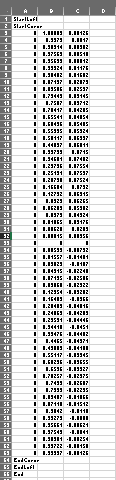
\includegraphics[width=0.3\textwidth]{points.png}
	\caption{Listado de puntos del perfil alar.}
\end{figure}

Una vez que cargamos estos puntos en las hojas de cálculo procedemos a utilizar el macro específico para CATIA, ya que ahí realizaremos el modelo y la simulación de nuestro perfil alar.

\begin{figure}[H]
	\centering
	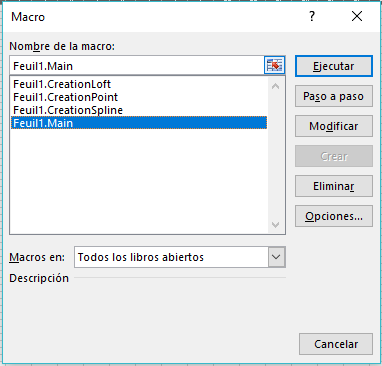
\includegraphics[width=0.5\textwidth]{macro.png}
	\caption{Elección del macro a utilizar.}
\end{figure}

Una vez que hemos hecho esto, una serie de puntos apareceŕán en un plano de nuestra elección en el software de CATIA. Si nos encargamos de reordenar éstos y generar la extrusión para poder visualizar nuestro perfil alar obtendremos la siguiente figura tridimensional.

\begin{figure}[H]
	\centering
	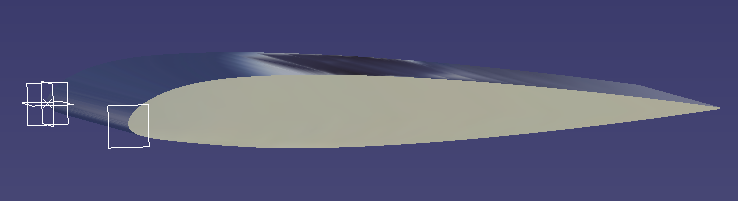
\includegraphics[width=0.8\textwidth]{perfil.png}
	\caption{Perfil alar después de haber importado los puntos de las hojas de cálculo.}
\end{figure}

Teniendo este modelo, es posible ver cómo actuarían distintas fuerzas, para el siguiente análisis se utilizó la opción de análisis de presiones. En este caso utilizamos una presión de 500 Pa  y obtuvimos las siguientes imágenes.

\begin{figure}[H]
	\centering
	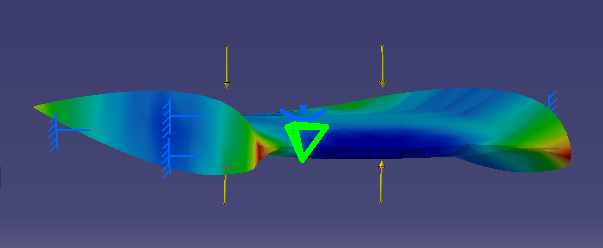
\includegraphics[width=0.8\textwidth]{forces.png}
	\caption{Fuerzas aplicadas de manera distributiva.}
\end{figure}

\begin{figure}[H]
	\centering
	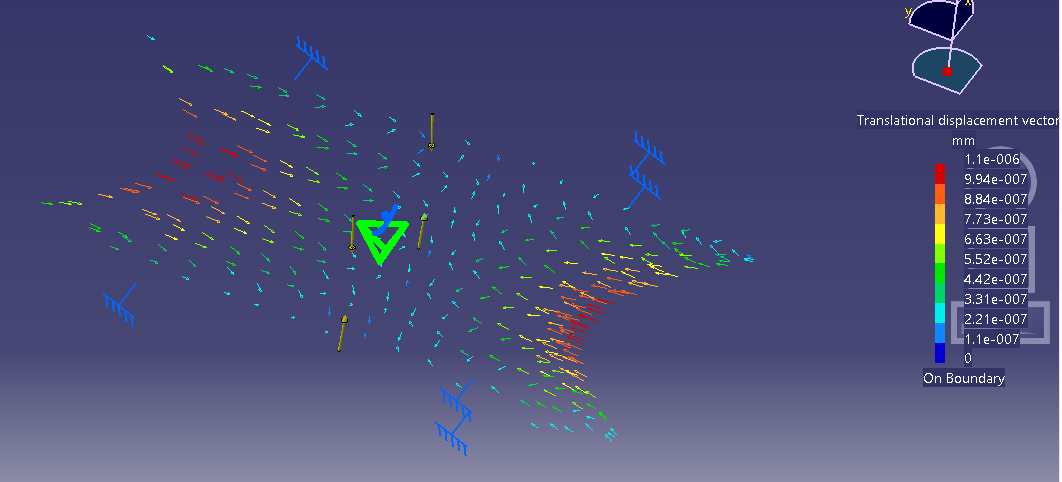
\includegraphics[width=0.8\textwidth]{vector.png}
	\caption{Fuerzas internas que experimenta el ala.}
\end{figure}

\begin{figure}[H]
	\centering
	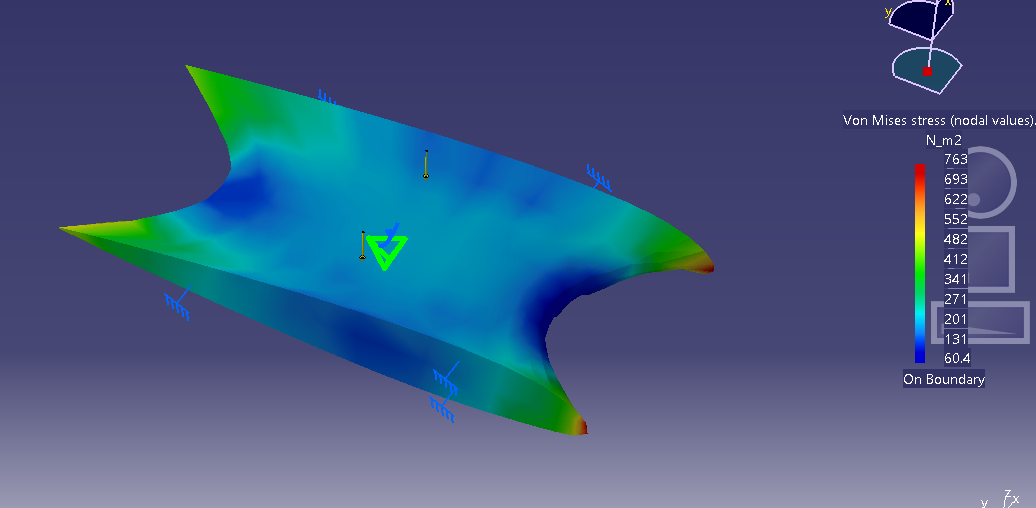
\includegraphics[width=0.8\textwidth]{vonmises.png}
	\caption{Análisis de von Mises para las fuerzas que se aplican.}
\end{figure}

\section*{Conclusión}

Podemos observar cómo esta presión afecta al ala, esto nos puede ser de mucha ayuda al momento de diseñar sistemas que soporten grandes fuerzas, también el material por utilizar puede ser propenso a cambios si las propiedades de éste resultan uy inconvenientes a comparación de otro.
%%%%%  Bib
\renewcommand\refname{Referencias}
\printbibliography
\end{document}
